%=================================
%====template for LATEX poster==== 
%=================================

%--A0 beamer slide--
\documentclass[final]{beamer}
%\usepackage[orientation=portrait,size=a0,
%            scale=1.25         % font scale factor
%        ]{beamerposter}

% modify for 36x48in poster
\usepackage{beamerposter}
\setlength{\paperwidth}{48in}
\setlength{\paperheight}{36in}

\geometry{
  hmargin=2.5cm, % little modification of margins
}

%
\usepackage[utf8]{inputenc}

\linespread{1.15}
%
%==The poster style============================================================
\usetheme{sharelatex}

%==Title, date and authors of the poster=======================================
\title
[Gulf of Mexico Oil Spill \& Ecosystem Science Conference, February 5--10 2017, New Orleans, USA] % Conference
{ % Poster title
A Dynamical Geography of the Gulf of Mexico
}

\author{ % Authors
P. Miron\inst{1}, %, Author Two\inst{2}, Author Three\inst{2,3}
F. J. Beron-Vera\inst{1},
M. J. Olascoaga\inst{1},
 Paula P\'erez-Brunius\inst{2}, 
 Julio Sheinbaum\inst{2} and 
 Gary Froyland\inst{3}
}
\institute
[Very Large University] % General University
{
\inst{1} Rosenstiel School of Marine and Atmospheric Science, University of Miami, USA
\\[0.3ex]
\inst{2} CICESE, Ensenada, Mexico
\\[0.3ex]
\inst{3} University of New South Wales, Sydney, Australia
}
\date{\today}

% other useful packages
\usepackage[super,sort&compress]{natbib}
\usepackage{siunitx}
\usepackage{tikz}
\newcommand{\PF}{\mathcal{P}}
\newcommand{\ia}{\textit{a}}
\newcommand{\ib}{\textit{b}}
\newcommand{\ic}{\textit{c}}
\newcommand{\id}{\textit{d}}
\newcommand{\ie}{\textit{e}}
\newcommand{\gom}{GoM}
\let\vaccent=\v 
\renewcommand{\v}[1]{\ensuremath{\mathbf{#1}}} 
\newcommand{\minus}{\scalebox{0.5}[1.0]{$-$}}


\begin{document}
\begin{frame}[t]
\begin{multicols}{3}

% The poster content
\section{Introduction}
Density dispersion in fluid flow is difficult to predict as it involves many mechanisms affecting a wide range of time and length scales. In the present study, we use the available drifter trajectories database (from 1994--2016) to extract almost-invariant regions and predict transport in the Gulf of Mexico (\gom). A total of 3207 drifter trajectories from several sources were considered and all the data points are presented in Fig.~\ref{fig:gom}. These drifters were deployed over many years and their design differs from experiment to experiment, so some variations in their Lagrangian properties can be expected.  For the purposes of this work, these variations are ignored as the main goal is the analysis of the average dynamics of the \gom.
\begin{figure}
\centering
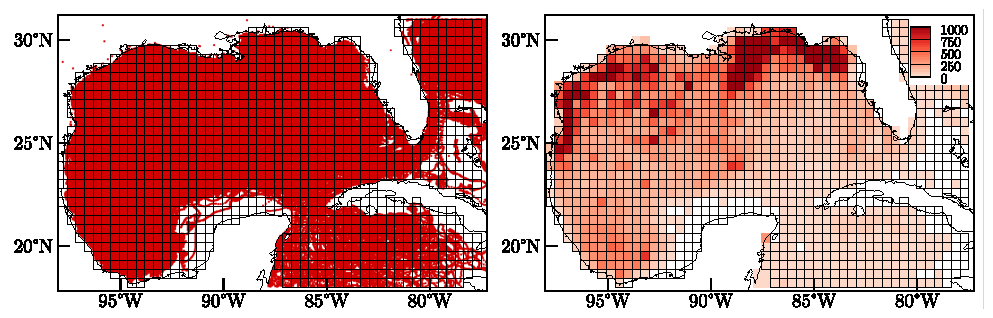
\includegraphics[width=0.9\columnwidth]{figures/fig03}
\caption{All data points of drifter trajectories are plotted on the left panel and the drifters density in each bin (from 1-4266 data points per bin with an average of 246) is presented on the right panel.}
\label{fig:gom}
\end{figure}

\section{Method}
The eigenvector method\citep{froyland2014well} employed is rooted in Markov-chain concepts that have led to the possibility of approximating invariant sets in dynamical systems using short-run trajectories\citep{dellnitz1997almost}. The dynamical system of interest is that governing the motion of the fluid particles, which are described by satellite-tracked drifters on the ocean surface.

Let $X$ be a closed 2D flow domain and denote by $T(x)$ the end point of a trajectory starting at $x \in X$ after some short time. A discretization of the dynamics can then be attained using Ulam's method\citep{ulam1960,Froyland-01} by dividing the domain $X$ into $N$ boxes $\left(B_1,\cdots,B_N\right)$. The probability of going from a box  $B_i$ to a box $B_j$ under one application of $T$ is (approximately) equal to
\begin{equation*}
 \PF_{ij} \approx \frac{\#\lbrace d: d \in B_i \text{ and } T(d) \in B_j\rbrace}{\#\lbrace d \in B_i\rbrace} \text{ with } d \text{ the individual drifter.}
\end{equation*}

The transition matrix $\PF$ defines a Markov Chain of the dynamics, which is a stochastic model describing a sequence of possible events in which the probability of each event depends only on the current state. From an initial density $f_0$, future distribution can be approximate by $\mathbf{f}_k = \mathbf{f}_0 \PF^k$.

The left eigenvector ($\lambda L = L \PF$) with $\lambda = 1$ describes the limiting distribution of the system while the corresponding right eigenvector is supported on the basin of attraction of the distribution.  Furthermore, eigenvectors associated with eigenvalues smaller than one allow the extraction of almost-invariant sets, which are relevant in dynamical systems governing motion that exhibits transient behavior.

\subsection{Example using a reduced Markov chain}
\begin{figure}[!ht]
  \centering
  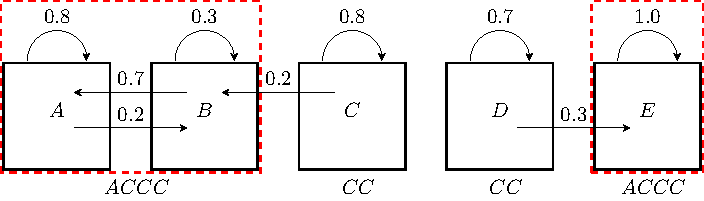
\includegraphics[width=0.8\columnwidth]{figures/fig01}
  \caption{The probability of moving from one state to another and if a state or group of states belongs to a communicating class (CC) or an absorbing closed communicating class (ACCC) are identified.}
  \label{fig:ccc}
\end{figure}
On the associated transition matrix, there is one line for each state of the system and the values in each column represents the probability of going from state $i$ to state $j$.  

\vspace{0.5cm}
\columnbreak
From left eigenvectors $L_{1-2}$, one can identify both ACCC $\lbrace A, B\rbrace$ and  $\lbrace E \rbrace$ while their respective basins of attraction are identified by the corresponding right eigenvectors $R_{1-2}$.

\begin{equation*}
\PF = 
  \begin{tabular}{c|ccccc}
    & A & B & C & D & E\\\hline
  A & 0.8 & 0.2 & 0 & 0 & 0\\
  B & 0.7 & 0.3 & 0 & 0 & 0\\
  C & 0 & 0.2 & 0.8 & 0 & 0\\
  D & 0 & 0 & 0 & 0.7 & 0.3\\
  E & 0 & 0 & 0 & 0 & 1.0
  \end{tabular}\quad
  L_1^T = 
  \begin{pmatrix}
  0.83\\
  0.55\\
  0\\
  0\\
  0
  \end{pmatrix}\quad
  R_1 = 
  \begin{pmatrix}
  1\\
  1\\
  1\\
  0\\
  0
  \end{pmatrix}\quad
  L_2^T = 
  \begin{pmatrix}
  0\\
  0\\
  0\\
  0\\
  1
  \end{pmatrix}\quad
  R_2 = 
  \begin{pmatrix}
  0\\
  0\\
  0\\
  1\\
  1
  \end{pmatrix}
\end{equation*}

\section{Results and discussions}
The eigenvector method is now applied to the transition matrix $\PF$ constructed from the drifter trajectories using a 2 day transition time. The left eigenvector associated with the largest eigenvalue less than one identifies the main attractor (Fig.~\ref{fig:l_eig}\ia) on the right part of the domain, communicating with the Atlantic Ocean. The associated right eigenvector (Fig.~\ref{fig:r_eig}\ia) covered the whole domain as stated by the Perron--Frobenius theory, except from the small isolated close communicating classes (CCC). This states that with the global circulation of the Gulf of Mexico, any density is diluted, trapped by the Loop Current into the Florida Strait and evacuated to the Atlantic Ocean.

\begin{figure}
\centering
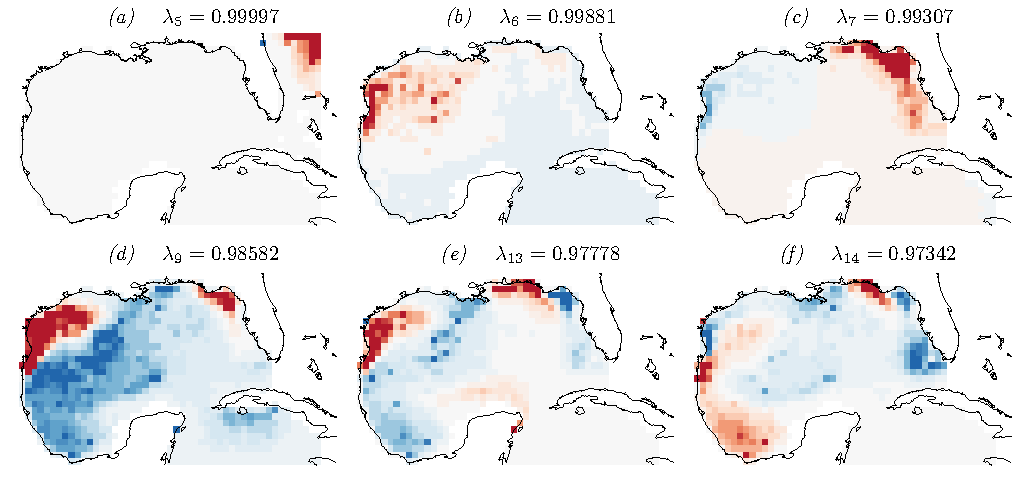
\includegraphics[width=\columnwidth]{figures/fig06}
\caption{Left eigenvectors showing the principal attractive regions.}
\label{fig:l_eig}
\end{figure}

 Fig.~\ref{fig:l_eig}\ib\ identifies the main attractor inside the \gom. It is located on the western boundary of the \gom\ on the Tamaulipas (Mexico) Gulf Coast while its basin of attraction (Fig.~\ref{fig:r_eig}\ib) splits the \gom\ in two at the west of the Yucat\'{a}n Channel. 
 
 Fig.~\ref{fig:l_eig}\ic\ highlights an attractive region on the West Florida Shelf while the next eigenvectors (bottom of Fig.~\ref{fig:l_eig}) emphasize on the presence of 4 different attractors; on  the south shore of Cuba, the SW coast of the \gom, at the northern part of the West Florida Shelf and on the NW shore of the \gom\ on the Texas Gulf Coast.
\begin{figure}
\centering
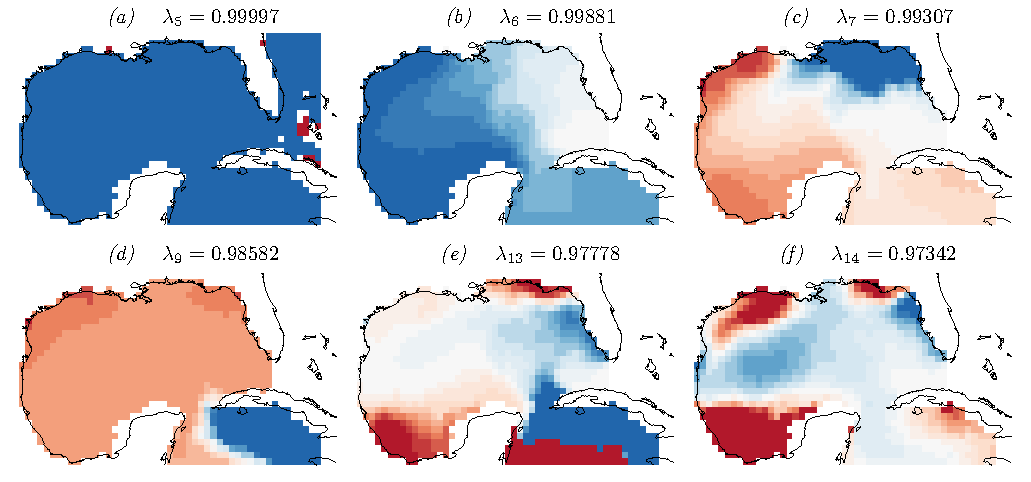
\includegraphics[width=\columnwidth]{figures/fig07}
\caption{Right eigenvectors showing the corresponding basins of attraction of the attractive regions in Fig.~\ref{fig:l_eig}.}
\label{fig:r_eig}
\end{figure}

\vspace{0.5cm}
\columnbreak
\subsection{Dynamical geography}
The dynamical geography is a partition of the surface of the \gom\ developed by combining the basins of attraction presented in Fig.~\ref{fig:r_eig}. On the left, the \gom\ is split into two regions, one connecting the Caribbean Sea to the Atlantic while the other is isolated on the western side. The separation of the \gom\ fit well with the boundary of the Loop Current, identified in diverse papers\citep{maze2015historical}. On the right, five weakly interacting coastal basins are extracted by thresholding the support area of the right eigenvectors. Each coastal basin is characterized by a distinct flow dynamics and coherence for important time scale. Those regions are consistent with observations of slow dynamics around the Mississippi Delta, of more intensively mixing region around the Florida Coast and of transient eddy structures south of the Island of Cuba.
\begin{figure}
\centering
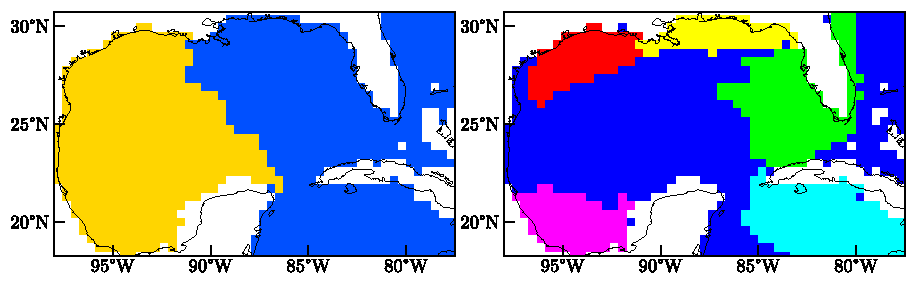
\includegraphics[width=0.95\columnwidth]{figures/fig09}
\end{figure}

The transition matrix $\PF$ can also be used to predict the dispersion of passive tracers such as oil spills (Fig.~\ref{fig:oil}). Each row shows the evolution of  two distinct oil spills, one occurring in a coastal basin and the other one further away from the coast. While the top row density stays mostly inside the basin during all the \SI{36}{d} period, the bottom row evolution presents a wider spread due to the increased mixing and transport further away from the coast.

\begin{figure}
\centering
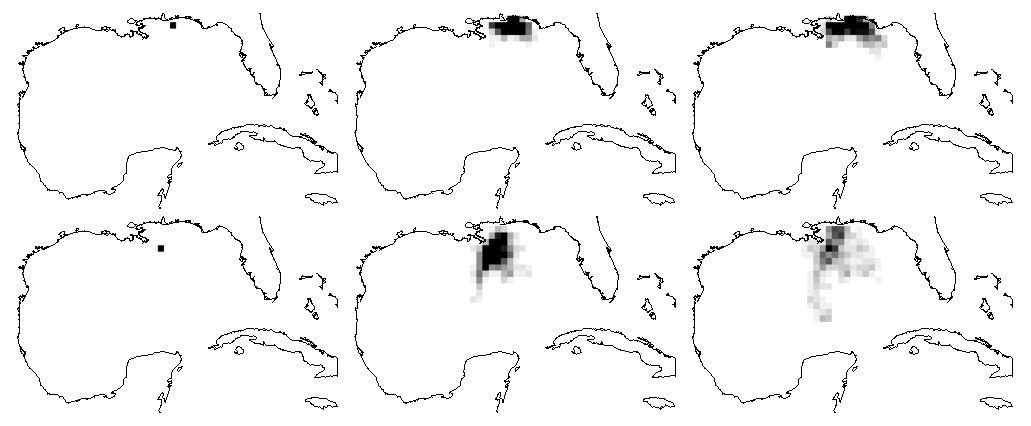
\includegraphics[width=0.9\columnwidth]{figures/fig_oil}
\caption{Each row presents the evolution of two different oil spills inside the \gom. The left column shows the initial location of the density while the 2nd and 3rd columns present the evolution after 16 and 36 days.}
\label{fig:oil}
\end{figure}

\section{Conclusions}
We construct a Markov-chain representation of the surface-ocean Lagrangian dynamics in the region spanned by the \gom\ and the northern Caribbean Sea using a very large collection of drifter trajectories. From the analysis of the eigenvalues and eigenvectors of the transition matrix associated with the chain, we identify almost-invariant attracting sets and their basins of attraction. With this information, we decompose the GoM's geography into weakly dynamically interacting provinces in both forward and backward time, which has implications for the connectivity of passive (Lagrangian) and potentially also non-passive (e.g., chemically reacting, biologically active) tracers in the \gom. 

%\subsection{References}

\bibliographystyle{abbrvnat}
% remove References title
\begingroup
\renewcommand{\section}[2]{}%
% add cited papers
\small{\bibliography{references,fot}}
\endgroup
\vspace{0.5cm}
\end{multicols}
\end{frame}
\end{document}